% Rod1717 with 170 layers         
\begin{figure*} \centering
      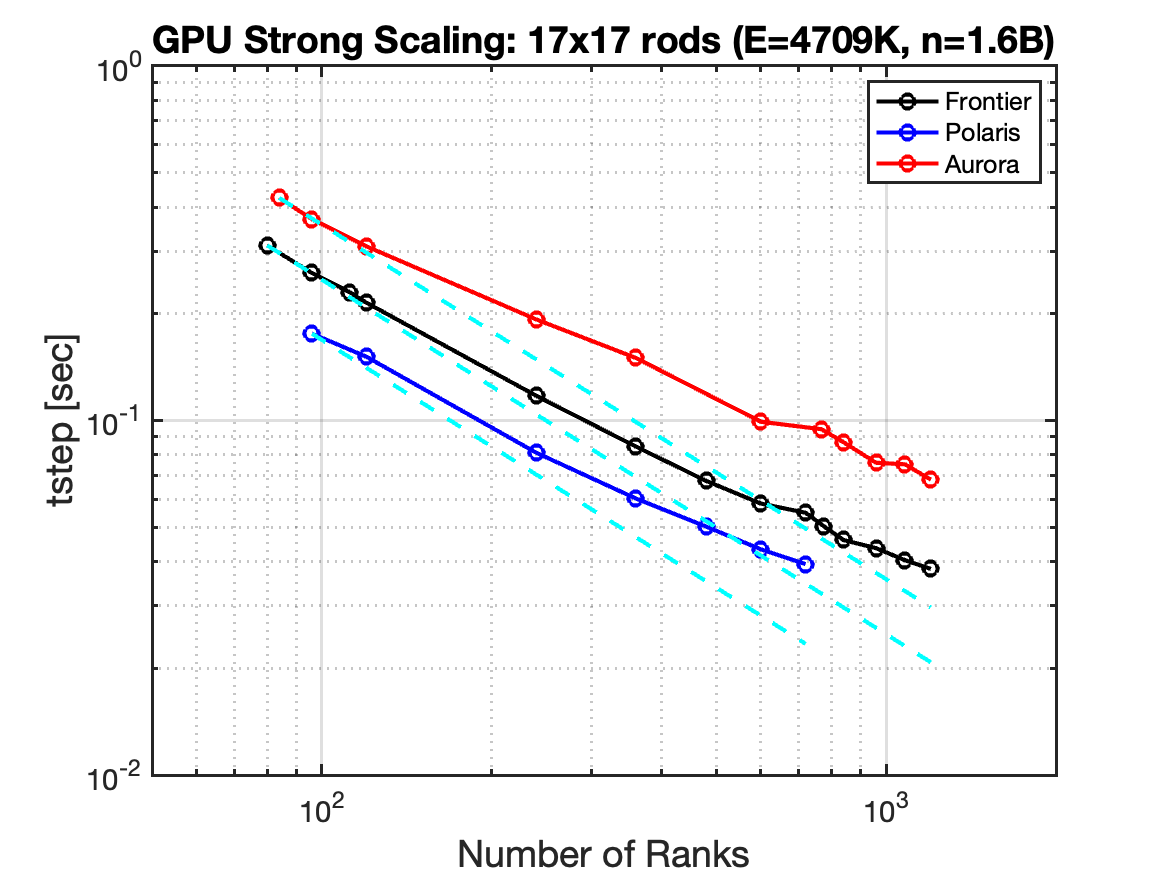
\includegraphics[width=3.1in]{figs/strong-scale-rod1717-170-p-rank-gmpi-all-frontier-aurora-0318.png}
      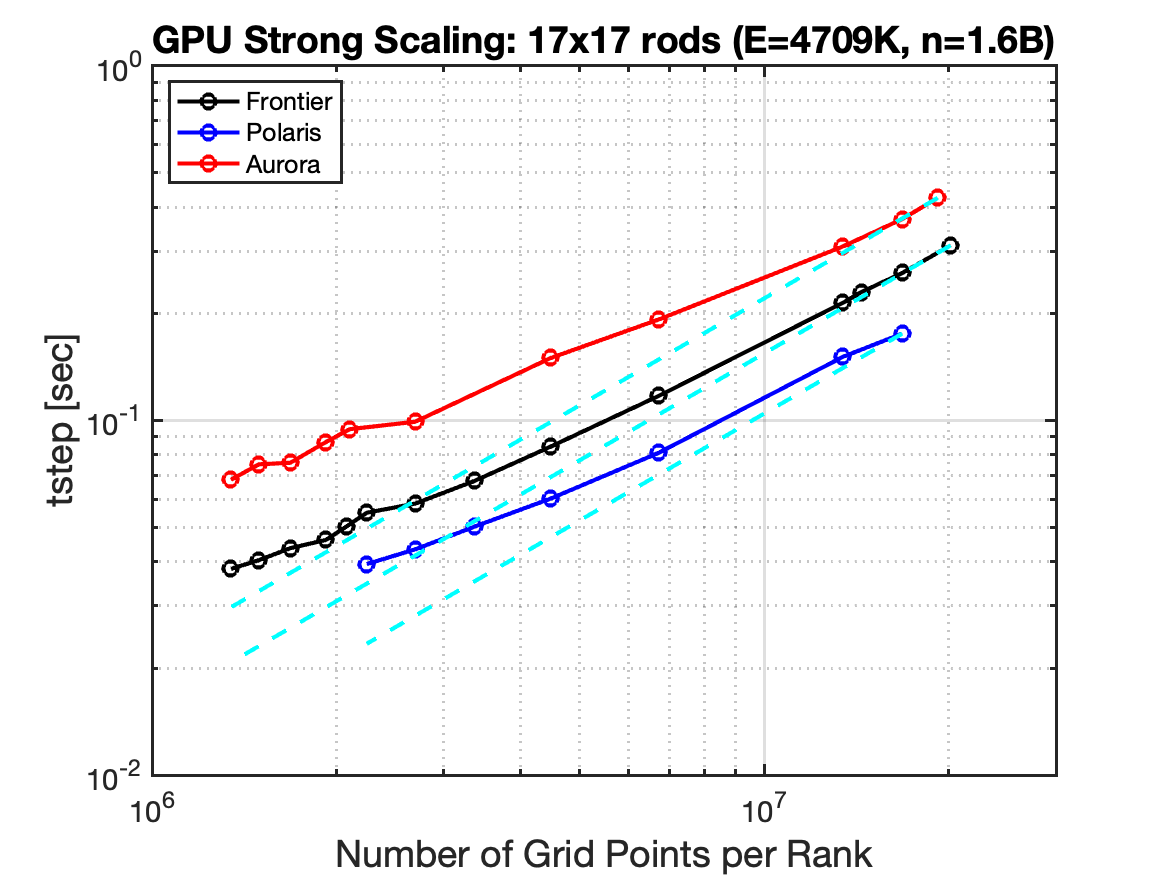
\includegraphics[width=3.1in]{figs/strong-scale-rod1717-170-n-p-rank-gmpi-all-frontier-aurora-0318.png}
      \\
      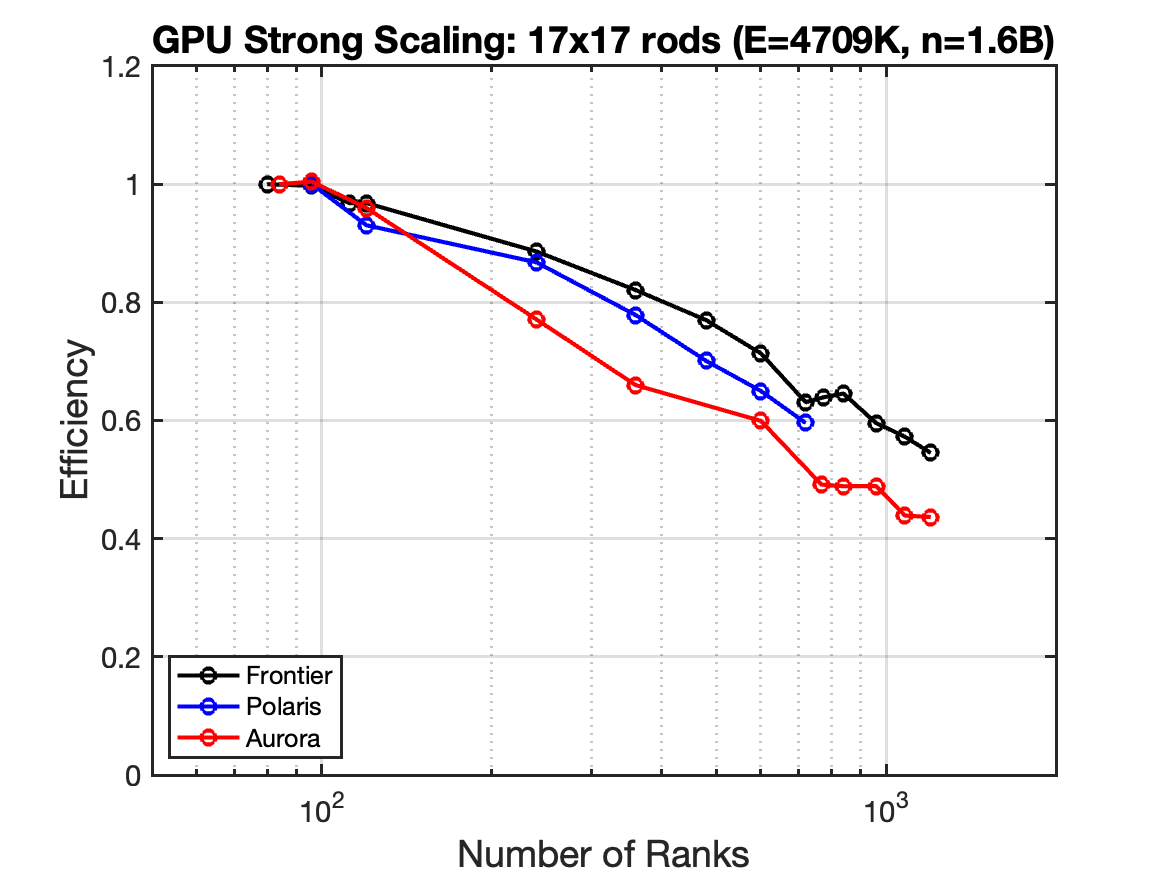
\includegraphics[width=3.1in]{figs/strong-scale-eff-rod1717-170-p-rank-gmpi-all-frontier-aurora-0318.png}
      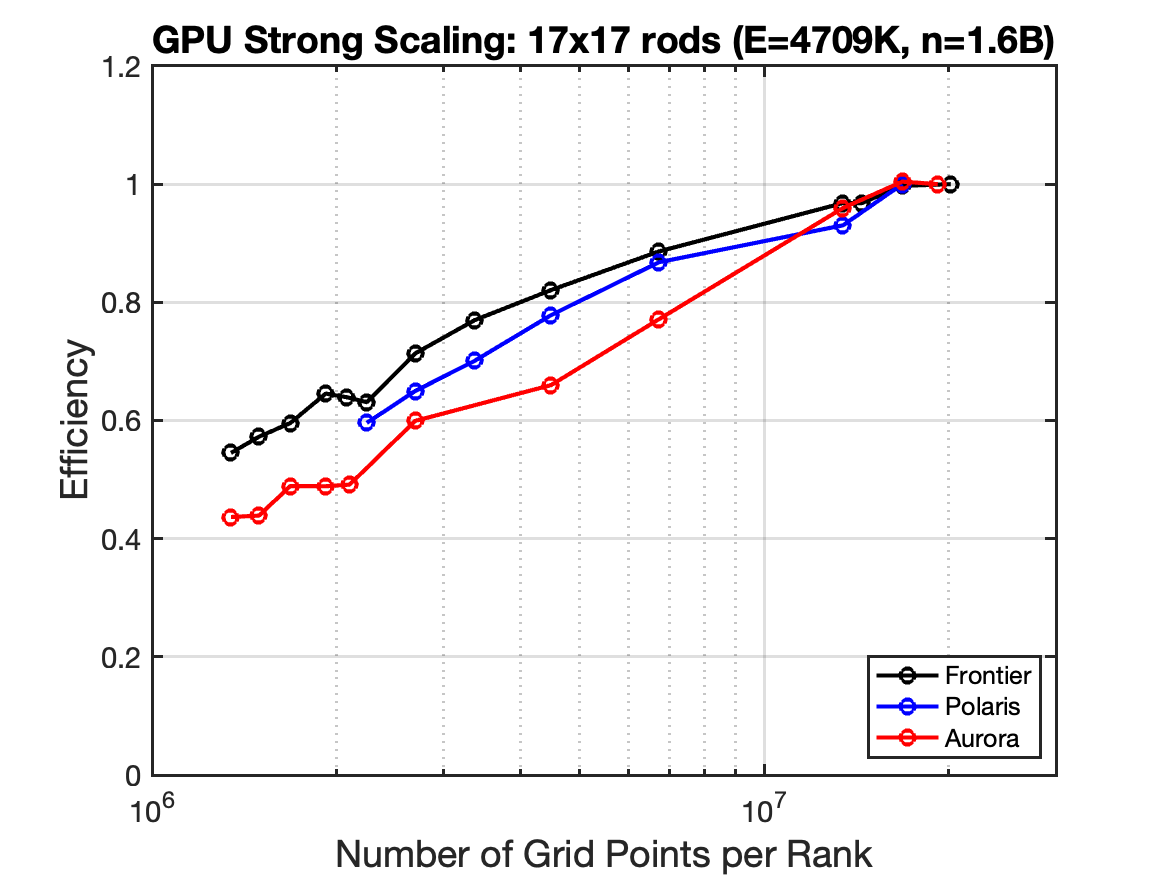
\includegraphics[width=3.1in]{figs/strong-scale-eff-rod1717-170-n-p-rank-gmpi-all-frontier-aurora-0318.png}
      \\
      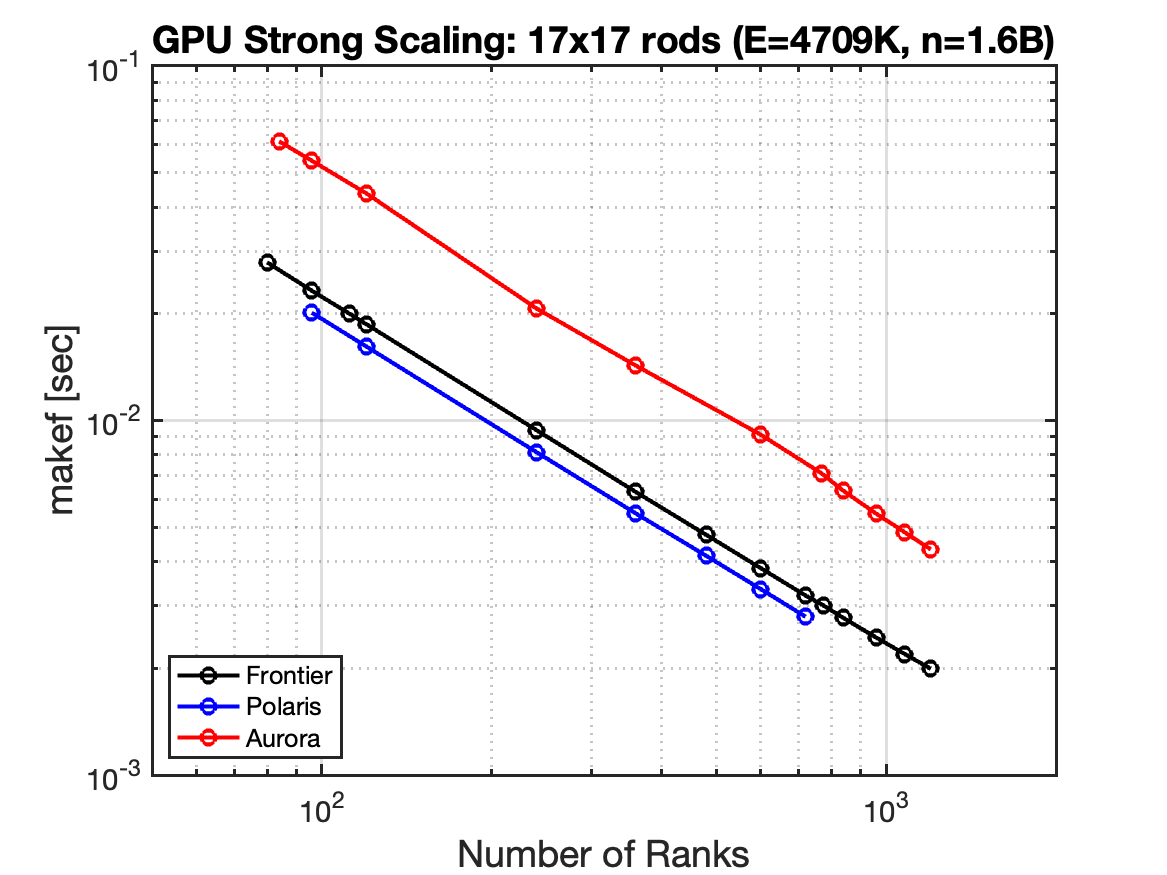
\includegraphics[width=3.1in]{figs/strong-scale-makef-rod1717-170-p-rank-gmpi-all-frontier-aurora-0318.png}
      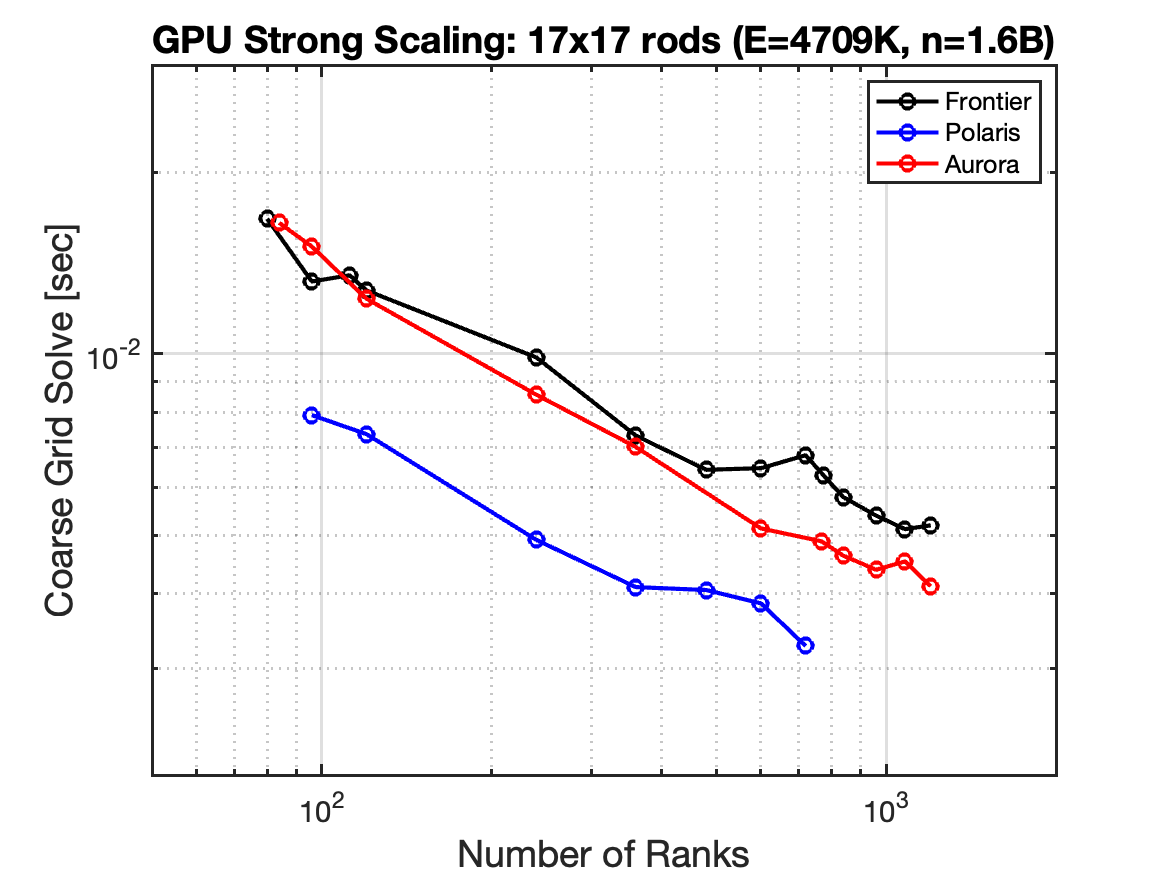
\includegraphics[width=3.1in]{figs/strong-scale-crs-rod1717-170-p-rank-gmpi-all-frontier-aurora-0318.png}
% \caption{\label{fig:rod1717-170-scale} Aurora, Frontier, and Polaris strong-scaling 
  \caption{\label{fig:scale} Aurora, Frontier, and Polaris strong-scalings 
            for Navier-Stokes simulation of $17\times 17$ rod bundle using the total number of
            grid points, $n=1.6B$.
            The average (wall) time per step, tstep, in seconds is measured over steps 1001--2000.
            makef is a routine responsible for setting up the right-hand-sides for the momentum equations, 
            involving evaluation of the dealiased advection operator for the velocity.}
\end{figure*}

